\graphicspath{{figs/}} %path to images
\chapter{Implementation (draft)}
\label{ch:lr}
\chaptermark{Fourth Chapter Heading}

\definecolor{codegreen}{rgb}{0,0.6,0}
\definecolor{codegray}{rgb}{0.5,0.5,0.5}
\definecolor{codepurple}{rgb}{0.58,0,0.82}
\definecolor{backcolour}{rgb}{0.95,0.95,0.92}

\lstdefinestyle{mystyle}{
    basicstyle=\ttfamily\footnotesize,
    backgroundcolor=\color{gray!10},
    frame=lines
}
\lstset{style=mystyle}


The following chapter provides implementation details for the system, including some issues that arose during development and the solutions to these issues.

\section{Component communication}\label{sec:communication}


\section{Entity-Relationship Diagram}

\begin{figure}[t]
    \centering
    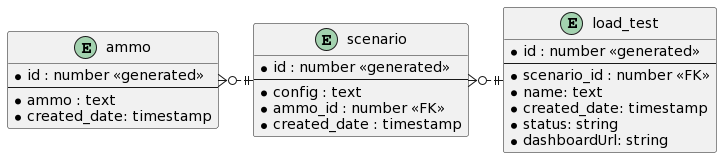
\includegraphics[height=\textheight,width=\textwidth,keepaspectratio]{erl.png}
    \caption{Entity-Relationship Diagram}
    \label{fig:erl}
\end{figure}


\section{Execute test scenario}

\begin{figure}[t]
    \centering
    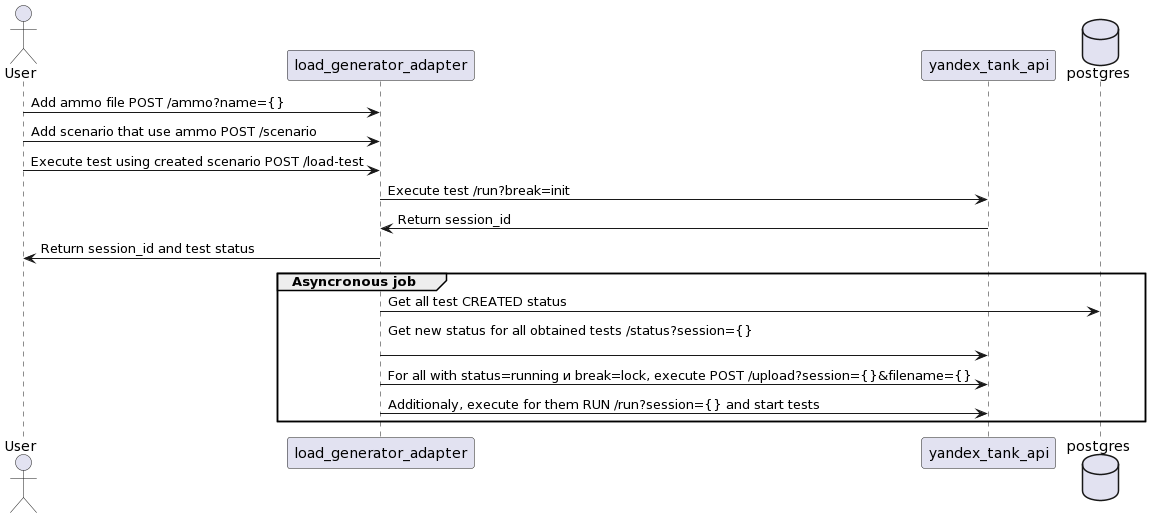
\includegraphics[height=\textheight,width=\textwidth,keepaspectratio]{diagram.png}
    \caption{Execute test scenario}
    \label{fig:test_scenario}
\end{figure}


\lstinputlisting[language=yaml]{code/docker-compose.yaml}

To visualize text as code in monospace font in LaTeX, you can use the `listings` package. The `listings` package provides a way to display code snippets and offers various customization options. Here's an example of how you can use it:

\begin{lstlisting}[language=XML, style=mystyle]
    fun helloWorld() {
        println("Hello, World!")
    }
\end{lstlisting}